\documentclass{standalone}
\usepackage{tikz}
\begin{document}
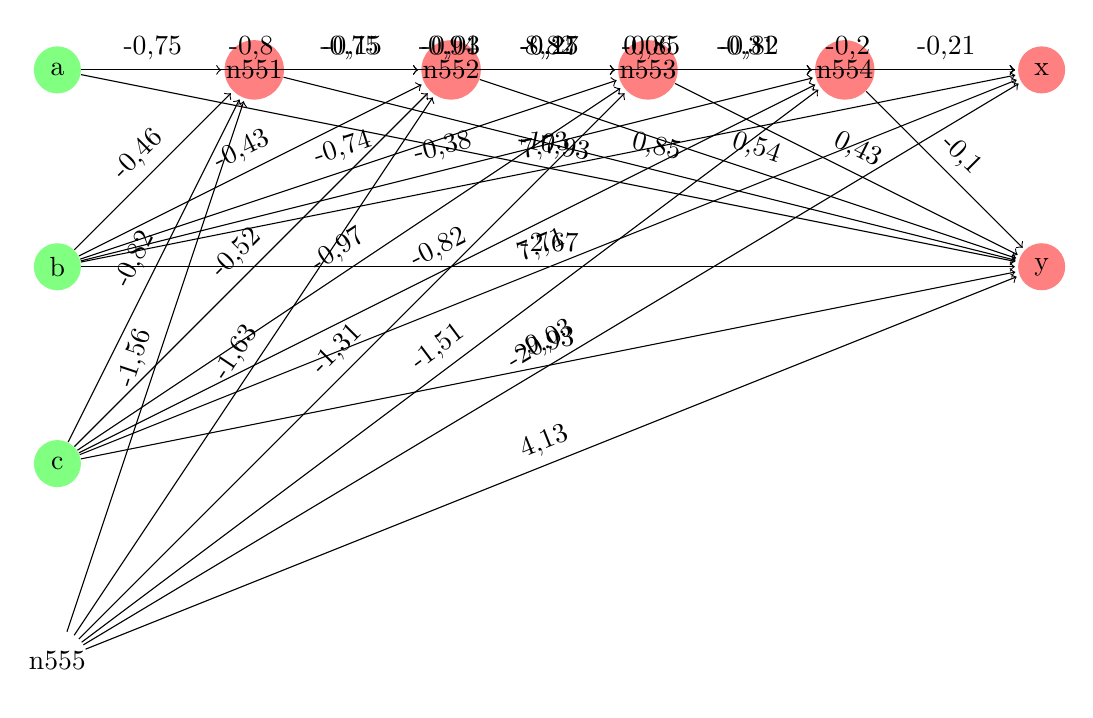
\begin{tikzpicture}[shorten >=1pt,->,draw=black!,node distance=2.5cm]
\tikzstyle{neuron}=[circle,fill=black!25,minimum size=17pt,inner sep=0pt]
\tikzstyle{constant}=[neuron, fill=white!50];
\tikzstyle{sigmoid}=[neuron, fill=red!50];
\tikzstyle{identity}=[neuron, fill=green!50];
\node [identity] (a) {a};
\node [identity,below of=a] (b) {b};
\node [identity,below of=b] (c) {c};
\node [constant,below of=c] (n555) {n555};
\node [sigmoid,right of=a] (n551) {n551};
\node [sigmoid,right of=n551] (n552) {n552};
\node [sigmoid,right of=n552] (n553) {n553};
\node [sigmoid,right of=n553] (n554) {n554};
\node [sigmoid,right of=n554] (x) {x};
\node [sigmoid,below of=x] (y) {y};
\path[every node/.style={sloped,anchor=south,auto=false}]
(n554) edge node {-0,21} (x)
(n554) edge node {-0,1} (y)
(n553) edge node {-0,2} (x)
(n553) edge node {0,43} (y)
(n553) edge node {-0,31} (n554)
(n555) edge node {-20,03} (x)
(n555) edge node {-1,56} (n551)
(n555) edge node {4,13} (y)
(n555) edge node {-1,31} (n553)
(n555) edge node {-1,63} (n552)
(n555) edge node {-1,51} (n554)
(b) edge node {7,73} (x)
(b) edge node {-2,67} (y)
(b) edge node {-0,46} (n551)
(b) edge node {-0,43} (n552)
(b) edge node {-0,74} (n553)
(b) edge node {-0,38} (n554)
(a) edge node {8,82} (x)
(a) edge node {-0,94} (n554)
(a) edge node {-10,93} (y)
(a) edge node {-0,75} (n551)
(a) edge node {-0,8} (n552)
(a) edge node {-0,75} (n553)
(n552) edge node {-0,82} (x)
(n552) edge node {0,54} (y)
(n552) edge node {-0,27} (n553)
(n552) edge node {0,06} (n554)
(c) edge node {7,71} (x)
(c) edge node {-9,93} (y)
(c) edge node {-0,82} (n551)
(c) edge node {-0,52} (n552)
(c) edge node {-0,97} (n553)
(c) edge node {-0,82} (n554)
(n551) edge node {-0,85} (x)
(n551) edge node {0,85} (y)
(n551) edge node {-0,15} (n552)
(n551) edge node {-0,03} (n553)
(n551) edge node {-0,15} (n554)
;\end{tikzpicture}
\end{document}